\chapter{系统设计}
\label{cha:system_design}

\section{设计目标与需求分析}
\label{sec:design_goals}

OpsEvolver 的设计目标不是构建一个只能在固定数据集上完成根因分类的模型，而是构建一个能够进入真实云原生环境、借助工具链与环境交互、并通过演练持续学习的原型系统。围绕这一目标，本文将系统需求概括为以下四点。
\begin{enumerate}
    \item \textbf{自主诊断能力。} 当系统出现告警时，智能体应能够基于有限上下文快速组织检查路径，自主调用日志、指标、链路和命令行工具完成根因定位。
    \item \textbf{环境适配能力。} 系统应能够从特定业务环境中积累知识，使诊断决策不再完全依赖通用模型的先验，而是逐步吸收本地拓扑、服务命名和故障经验。
    \item \textbf{安全可控的演练能力。} 为避免智能体执行不受约束的危险操作，故障注入动作需要被限制在可声明、可回滚、可追溯的受控集合中。
    \item \textbf{持续演化能力。} 在线诊断不是系统的终点，诊断成功与失败都应转化为结构化反馈，用于修正知识库、更新规则并指导下一轮离线演练。
\end{enumerate}

从系统工程角度看，上述需求意味着 OpsEvolver 既要具备典型 Agent 的“推理+工具调用”能力，也要具备运维系统所要求的“状态持久化+历史回放+知识追踪”特征。因此，本文采用“工作流驱动、多智能体协作、知识外置存储”的总体设计思路。

\section{方法论原则}
\label{sec:methodology_principles}

结合当前原型系统的迭代结果，OpsEvolver 的方法论可以进一步概括为三个互相支撑的原则。

\subsection{主动学习：通过故障演练制造高价值样本}

传统告警驱动系统只能被动等待故障发生，样本稀缺且分布高度受生产流量影响。OpsEvolver 则通过混沌工程主动向环境施加扰动，将“系统可能出问题的地方”转化为可观测、可复盘、可沉淀的离线样本。对 SRE 智能体而言，主动演练的意义不在于单次注入本身，而在于把隐含的运维经验转化为结构化知识：哪些故障能够产生明显告警、哪些故障只在上游服务中体现、哪些故障会诱发误导性日志，都会在演练过程中逐步暴露出来。

进一步地，当前系统还显式记录“无告警注入”集合。也就是说，当某一类故障在当前负载和采样条件下没有形成可观测异常时，系统不会简单地把该轮实验视为失败，而是把它作为一类特殊知识保存下来，用于约束后续探索空间。这使主动学习过程不只是积累正样本，也在持续学习“哪些扰动在当前环境下不值得重复尝试”。

\subsection{可观测性感知：同时学习有效区域与无效区域}

传统故障演练往往只关心“有没有成功把故障注入进去”，但对智能运维系统而言，更关键的问题是“该故障是否真的在当前观测栈与工作负载下产生了可学习信号”。如果一次注入没有触发任何指标异常、链路退化或错误日志，那么它对当前阶段的诊断能力提升就十分有限。基于这一认识，OpsEvolver 在方法论上把可观测性边界也纳入学习目标，将无告警注入视作一种负样本，而不是简单丢弃。

这种做法带来两个直接收益。第一，系统能够显式识别当前实验设置下的“不可观测区域”，从而避免把预算反复消耗在短时间内难以产生告警的故障组合上。第二，后续实验分析不再只统计知识条目和成功案例，而能同时刻画哪些故障类型受限于负载、采样窗口或业务路径，尚未形成稳定的异常信号。换言之，OpsEvolver 学到的不仅是“什么故障会导致什么症状”，还包括“什么故障在当前环境里暂时学不到”。

\subsection{探索/利用分离：离线广覆盖，在线快收敛}

OpsEvolver 采用典型的 Explore/Exploit 分离思想。离线阶段强调覆盖面和多样性，允许智能体通过较高温度推理和更开放的探索策略尝试不同故障与诊断路径；在线阶段强调收敛速度和稳定性，尽量复用已沉淀的知识条目与规则库，减少重复探索。

这一分离策略的价值，在于把“学会环境”与“服务告警”两件事解耦。离线阶段承担环境适配与知识采样，在线阶段承担实时响应与知识利用。前者偏学习，后者偏执行，两者通过知识库、规则库和反馈闭环连接起来，使系统能够在长期运行中兼顾学习效率与响应效率。

\subsection{双系统认知：经验驱动与推理驱动协同}

从认知框架上看，OpsEvolver 具备明显的双系统特征。System 1 是外化的经验系统，主要由 KnowledgeBase 和 Rulebook 组成，负责提供先验模式、相似案例和高层排查习惯；System 2 是运行时的 Plan-Act-Observe-Reflect 推理循环，负责根据当前告警、现场观测和工具返回结果完成逐步判断。

这种设计避免了单纯依赖 LLM 即时推理的局限。经验系统用于压缩搜索空间，推理系统用于处理当前上下文中的细节与例外。若仅有 System 1，系统将退化为静态规则匹配；若仅有 System 2，系统又会在每次告警时从头探索。两者结合，才构成了面向真实运维环境的可持续演化机制。

\section{系统总体架构}
\label{sec:overall_architecture}

OpsEvolver 的整体架构如\autoref{fig:opsevolver-architecture}所示。系统以 Kubernetes 微服务环境为运行对象，以 Prometheus、Jaeger、日志接口和 Chaos Mesh 为外部支撑组件，并在上层构建离线演化、在线诊断和反馈闭环三个核心工作流。

\begin{figure}[htbp]
    \centering
    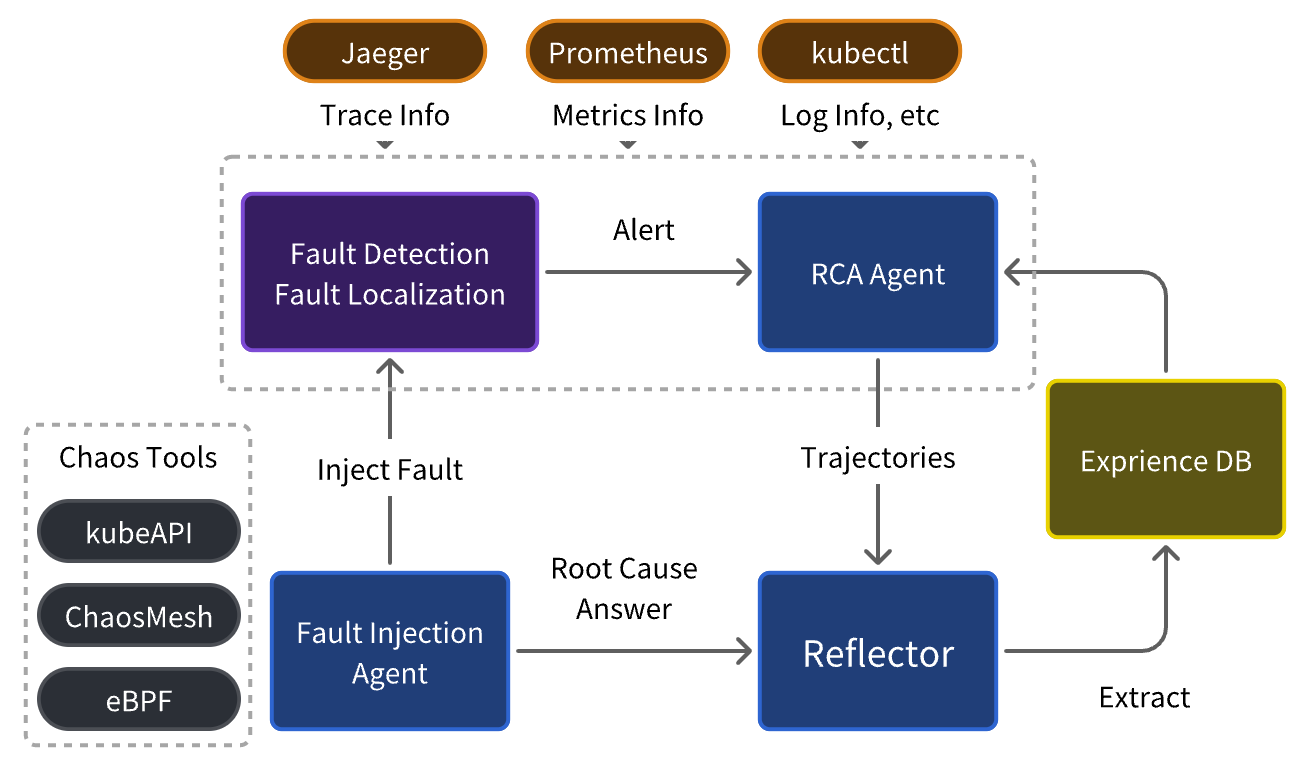
\includegraphics[width=0.78\textwidth]{image/proposal/architecture.png}
    \caption{OpsEvolver 原型系统总体架构}
    \label{fig:opsevolver-architecture}
\end{figure}

为便于说明，\autoref{tab:module-responsibility} 给出了系统中关键模块的输入、输出与职责划分。

\begin{table}[htbp]
    \centering
    \caption{OpsEvolver 关键模块职责划分}
    \label{tab:module-responsibility}
    \small
    \begin{tabular}{|p{2.6cm}|p{3.1cm}|p{3.1cm}|p{4.2cm}|}
        \hline
        模块 & 主要输入 & 主要输出 & 核心职责 \\ \hline
        ChaosExplorer & 命名空间拓扑、历史注入记录、故障动作集合 & 受控故障注入结果 & 选择未覆盖的故障动作并在目标环境中执行受控演练 \\ \hline
        AlertGenerator & 指标、链路、日志等遥测数据 & Alert 对象列表 & 监测故障注入后的可观测影响，生成统一告警描述 \\ \hline
        ExplorationDiagnoser & Alert、动作接口、探索提示词 & 诊断轨迹与诊断报告 & 在离线阶段尝试多路径诊断，为知识抽取提供原始轨迹 \\ \hline
        InferenceDiagnoser & Alert、知识条目、规则库 & 诊断轨迹与诊断报告 & 在在线阶段使用检索增强上下文快速定位故障 \\ \hline
        Introspector & 注入真值、告警、诊断轨迹 & 知识条目、规则库 & 对诊断过程进行评估，提炼可复用经验和通用规则 \\ \hline
        DeepThinker & 在线诊断结果、人工反馈或真值 & 失败类型与改进建议 & 分析失败原因，决定是否触发新一轮演化或修正规则 \\ \hline
        KnowledgeBase / HistoryBase & 知识条目、规则、周期记录 & 持久化文件 & 维护系统长期记忆，保证诊断与复盘过程可追踪 \\ \hline
    \end{tabular}
\end{table}

\subsection{离线演化工作流}

离线演化工作流承担“主动学习”的职责，是 OpsEvolver 与传统被动告警系统最本质的区别。其执行顺序可以概括为如下步骤。
\begin{enumerate}
    \item ChaosExplorer 根据当前命名空间内的服务和 Pod 拓扑、历史注入记录以及候选动作集合，选择一个尚未覆盖的故障动作。
    \item 系统执行故障注入后，由 AlertGenerator 在预设观察窗口中采集指标、日志与链路数据，若检测到异常则生成统一的 Alert 对象。
    \item ExplorationDiagnoser 面向该告警执行探索式诊断，形成包含多个动作与观测结果的诊断轨迹。
    \item Introspector 结合注入真值、告警信息和诊断轨迹，对诊断是否成功进行评估，并抽取知识条目与规则。
    \item 知识条目被写入知识库，注入记录、告警快照、轨迹摘要和生成规则被写入历史库，以支持后续追溯与重复注入规避。
\end{enumerate}

需要强调的是，离线演化中存在一个重要分支：如果故障注入后在观测窗口内没有触发任何异常告警，则该轮不会进入诊断与反思阶段，而是被记录为“无告警注入”。当前实现中，这类记录由 HistoryBase 独立持久化，并在下一轮故障选择时以 \texttt{no\_alert\_faults} 的形式回传给 ChaosExplorer，用于降低重复探索无效区域的概率。这一机制既反映了环境的可观测性边界，也为后续实验分析中的注入有效率统计提供了直接依据。

这一流程的关键价值在于，它为智能体提供了一个无需人工标注即可积累经验的机制。即使某次诊断未能完全命中真实根因，系统也能从失败样例中识别出知识盲区，为后续修正创造条件；而即便某次注入未形成告警，系统也能据此更新探索边界，从而避免盲目重复。

\subsection{在线诊断工作流}

在线诊断工作流对应真实生产告警的响应过程。相较于离线阶段，它不再执行故障注入与回收，也不再从零开始探索，而是尽量利用已有知识快速收敛。系统首先接收来自监控系统或告警生成器的 Alert，对当前告警进行上下文组装；随后从知识库中检索相似历史案例，并从规则库中筛选与当前告警最相关的规则，将两者与原始告警共同拼接为诊断提示；最后由 InferenceDiagnoser 执行低温度、低步数的推断式诊断。

在线工作流的核心目标是“在安全边界内尽快逼近正确答案”。因此它不强调探索多样性，而强调提示上下文的针对性和动作选择的简洁性。对于一个经过充分离线演化的环境，在线诊断理应优先重用已有经验，而不是重新发明排障路径。

\subsection{反馈闭环工作流}

反馈闭环位于离线演化与在线诊断之间，负责把线上真实案例重新送回学习过程。当在线诊断出现误判、低置信度结论或人工反馈指出错误时，DeepThinker 会分析失败类型，并生成对应的改进建议。如果问题属于分布外故障，则应触发新的故障演练；如果问题来自规则误导或知识检索错误，则需要调整规则优先级或知识条目置信度；如果问题来自数据缺失，则需要补充新的观测动作或更细粒度的遥测信息。

通过反馈闭环，OpsEvolver 不再是一次性推理系统，而是具备“经验回流”机制的演化系统。其本质是一种将线上故障样例持续转化为环境特定知识的工程化方案。

\section{多智能体协作机制}
\label{sec:multi_agent_collaboration}

\subsection{角色划分与职责边界}

OpsEvolver 并未采用单一全能型 Agent，而是通过角色专门化降低复杂任务的认知负担。ChaosExplorer 聚焦于故障设计与执行，主要解决“向环境施加什么扰动”的问题；Diagnoser 聚焦于告警后的证据搜集与根因推理，主要解决“发生了什么、为什么发生”的问题；Introspector 聚焦于对诊断过程的元分析，主要解决“此次诊断有哪些经验可沉淀”的问题；DeepThinker 则负责将在线失败映射为系统后续需要补足的学习任务。

这种分工方式具有两个直接好处。第一，不同角色可采用不同的提示词、温度参数和动作约束。例如探索阶段允许更强的发散性，而在线推断阶段则强调更低温度和更少步骤。第二，角色边界清晰后，系统更容易进行行为审计和结果解释，因为每一步动作都能被归因到特定模块。

\subsection{共享上下文与轨迹管理}

多智能体协作并不意味着任意共享长上下文。本文采用诊断轨迹与诊断报告作为核心中间表示：前者记录每一步的想法、动作、参数与观测结果，后者记录最终根因、置信度和证据链。对离线流程而言，Introspector 通过读取完整轨迹了解 Diagnoser 的决策过程；对在线流程而言，Feedback Loop 通过读取报告与轨迹判断诊断是否需要复盘。

这种“结构化状态共享”比直接共享原始聊天历史更稳定，原因在于它减少了冗长语义上下文带来的噪声，并使历史经验具备机器可检索、可比较的特征。系统中的 KnowledgeItem、CycleRecord 和 InjectionRecord 都建立在这种结构化共享思想之上。

\subsection{动作空间与执行约束}

为了将 Agent 的行为限制在可审计范围内，本文把可执行动作收敛为若干显式接口，例如获取日志、导出指标、读取链路、执行 shell 命令和提交结论等。动作空间的受控性体现在两个方面：其一，Agent 不能直接进行无限制的交互式命令操作，避免危险命令长驻执行；其二，故障注入动作必须来自预注册的 FaultAction 集合，且具备明确的参数校验与恢复路径。

因此，OpsEvolver 的自治并不是“完全放开”，而是在一组声明式工具能力内进行有边界的自主推理。这一设计兼顾了实验灵活性与系统安全性。

\section{知识表示与自演化机制}
\label{sec:self_evolve_mechanism}

\subsection{知识条目与规则库}

本文将离线演化产生的经验抽象为两类外部记忆。第一类是知识条目，面向具体症状模式，记录告警特征、推荐动作、适用条件、置信度以及所属演化周期；第二类是规则库，面向更通用的诊断经验，例如“网络异常应优先核查上下游依赖关系”或“高错误日志密度通常先于资源饱和出现”。知识条目更强调案例级复用，规则库更强调跨案例迁移。

与直接微调模型相比，这种外部记忆机制有两个优点：一是知识可以按条目增删改查，维护成本低；二是知识与原模型参数解耦，更适合快速迭代的云环境。系统不需要重新训练模型即可完成知识修正，只需更新知识库内容或规则优先级。

结合当前实现，知识条目与规则库还承担了“连接离线与在线”的中介角色。离线阶段每完成一轮演化，系统都会把新的知识条目和规则增量写入持久化存储；在线阶段则根据当前告警动态检索知识条目并装配规则提示。换言之，OpsEvolver 的学习结果并不隐藏在模型内部，而是以显式、可检查的形式不断生长。

除正向经验外，系统还通过历史库保存负向经验，即那些已经执行但未产生告警的故障组合。这部分信息虽然不会进入在线诊断的检索上下文，却会影响离线阶段的探索预算分配。因而，OpsEvolver 的“记忆”并不是单一知识库，而是由知识条目、规则库和负向探索边界共同构成的长期环境模型。

\subsection{上下文组装与相似案例检索}

在在线诊断阶段，InferenceDiagnoser 需要从已有知识中挑选最有价值的上下文。当前原型采用轻量级关键词匹配方法对历史知识进行排序，其打分思想可以写为
\begin{equation}
    \label{eq:retrieval-score}
    score(k_i, a)=2 \cdot \mathbf{1}[n(a)\in p_i]+\mathbf{1}[s(a)\in p_i],
\end{equation}
其中，$a$ 表示当前告警，$k_i$ 表示第 $i$ 条知识条目，$n(a)$ 表示告警名称，$s(a)$ 表示告警严重程度，$p_i$ 表示知识条目的症状描述文本，$\mathbf{1}[\cdot]$ 为指示函数。若告警名称与知识条目症状匹配，则给予更高权重；严重等级匹配则给予辅助加分。

尽管这一检索方法相对简单，但它体现了本文的重要设计原则，即“先通过外部记忆缩小诊断搜索空间，再让 LLM 在小范围内进行推理”。随着系统后续演进，该模块可以自然替换为向量检索或图检索，而不改变整体架构。

\subsection{失败分析与反馈触发}

DeepThinker 对失败样例的分析是自演化机制的核心。结合当前原型实现，系统重点关注以下几类失败。
\begin{enumerate}
    \item \textbf{规则误导（Rule Misleading）}：说明已有规则对当前场景并不适用，需要降低其优先级或补充反例。
    \item \textbf{错误知识检索（Wrong Knowledge Retrieved）}：说明检索阶段找到了相似但不正确的历史案例，需要修正知识条目置信度或相似度度量。
    \item \textbf{分布外故障（Out-of-Distribution）}：说明当前故障超出了知识库覆盖范围，应触发新的离线演化。
    \item \textbf{数据不完整（Incomplete Data）}：说明诊断过程中缺乏必要证据，需要新增观测动作或增强遥测采样。
    \item \textbf{超时（Timeout）}：说明当前诊断路径效率不足，需要压缩动作链路或优化工具执行性能。
\end{enumerate}

从机制上看，DeepThinker 并不直接替代 Diagnoser 的决策，而是作为元控制器对失败样本进行分类，并把“此次失败意味着系统缺什么”这一高阶问题转化为下一轮演练与知识更新的输入。

\section{系统设计特点与讨论}
\label{sec:design_discussion}

综合来看，OpsEvolver 的设计具有以下特点。其一，系统以工作流为组织核心，将故障注入、告警发现、证据搜集、知识提炼和反馈修正串联为端到端闭环，而非若干孤立模块。其二，系统采用“环境优先”的知识演化策略，强调针对特定业务系统逐步积累知识。其三，系统保留了较好的工程可扩展性，无论是新增故障动作、替换检索算法，还是引入新的遥测源，都可以在不重构整体架构的前提下完成。

当然，该设计也存在权衡。多工作流协作会带来更多持久化和状态管理开销；外部记忆方式虽然灵活，但质量高度依赖知识抽取模块的表现；离线演练的覆盖程度也将直接决定在线阶段的可迁移性。上述问题将在第四章实验与分析中进一步讨论。

\section{本章小结}
\label{sec:chap02_summary}

本章从需求分析、总体架构、多智能体协作、知识表示和失败反馈五个方面介绍了 OpsEvolver 的系统设计。通过将离线演化、在线诊断和反馈闭环统一到同一架构之下，本文为后续的工程实现和实验分析奠定了逻辑基础。下一章将进一步说明各模块在原型系统中的具体实现方式。
